\section{Results}
U
	Painting segmentation: 88.57 \% correct segmentation
	\todo{qualitative as well as quantitative}
	
	\todo{quantitative: graphs, tables, roc-curves, f1-scores, ...}
	
	\todo{qualititative: technisch, show where and why the method succeeds or fails, pictures of easy and difficulty cases}
	
	Because our method relies heavily on edge detection, there are cases where this could have a negative impact. In many cases, there is a shadow underneath the painting, as shown on figure \ref{fig:negative_case_shadow}.
	
	\begin{figure}
		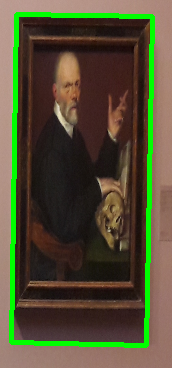
\includegraphics[width=\linewidth]{negative_case_shadow}
		\caption{An example of a shadow underneath the painting. This usually results in the segmentation algortihm to include this shadow as part of the painting because of the strong edge.}
		\label{fig:negative_case_shadow}
	\end{figure}

	\todo{stukje hierboven ook kwalitatief?}
This subsection, we will present a qualitative analysis of our algorithm. We will discuss its strengths, flaws and, with each point, present an example case to help as a visual aid. The flaws in particular help paint a picture of what can be done better in a future iteration of the algorithm. 
e do not deny its usefulness and believe that it may be beneficial to implement it in a future version of the algorithm \todo{waar nodig?, kan zijn dat ML gebruikt wordt bij matching}. Even though the algorithm's simplicity is presented as one of its strengths, it can also be considered as one of its weaknesses, much like a double edged sword.
match and detected keypoints between two runs. However, due to not detecting different potential candidate matches between runs results in the algorithm never being able to present a different solution for the given image.
 the matching function, but still manages to find a correct match.
lied to the building stage of the database.
ion phase detects such a painting and supplies it to the matching phase. A cascade of erroneous matches and room localizations may occur. The inverse is also true, as having an entry in the data set with few keypoints can result in a painting with many keypoints being wrongfully matched with a 'flat' one.
e descriptors of the segmented painting results in a total.
ion to this problem may lie in other journals \todo{ref naar boek/conference over bag of words/large databases}. \todo{laatste paragraaf herschrijven}